% Predstavitev seminarske naloge, NPMP 2026/27, skupina 08
% Prevajanje: latexmk -pdf predstavitev.tex
\documentclass[aspectratio=169,11pt]{beamer}

\usepackage[utf8]{inputenc}
\usepackage[T1]{fontenc}
\usepackage[slovene]{babel}
\usepackage{amsmath,amssymb}
\usepackage{graphicx}
\usepackage{booktabs}
\usepackage{tikz}
\usepackage{quantikz}

\usetheme[progressbar=frametitle,numbering=fraction]{metropolis}
\setbeamertemplate{navigation symbols}{}
\setbeamerfont{title}{size=\Large}

\graphicspath{{../porocilo/Skupina08/img/}}
\newcommand{\dobro}[1]{\textbf{\color{teal!70!black}#1}}
\newcommand{\slabo}[1]{\textbf{\color{red!70!black}#1}}

\title[Seštevalnika CDKM in Draper]{Primerjava kvantnih seštevalnikov CDKM in Draper (QFT) na šumnem kvantnem procesorju IBM}
\author{Jurij Anžič in Janez Koprivec}
\institute{Skupina 08 \\ Nekonvencionalne platforme in metode procesiranja}
\date{2026/27}

\begin{document}

\maketitle

% ---------------------------------------------------------------
\begin{frame}{Motivacija}
\begin{itemize}
  \item Seštevalnik je osnovni gradnik kvantne aritmetike \\
        {\small (Shor: modularno potenciranje $\rightarrow$ množenja $\rightarrow$ seštevanja)}
  \item Priročno merilo procesorja: pravilen rezultat je znan in je en sam izid
  \item Dve družini seštevalnikov:
  \begin{itemize}
    \item \textbf{CDKM}: reverzibilni zaporedni prenos, linearno mnogo vrat
    \item \textbf{Draper}: seštevanje v Fourierjevi bazi, kvadratno mnogo vrat
  \end{itemize}
  \item Pogosta predpostavka: \alert{manj dvokubitnih vrat $\Rightarrow$ uspešnejše vezje}
\end{itemize}
\end{frame}

% ---------------------------------------------------------------
\begin{frame}{Raziskovalno vprašanje in hipoteza}
\begin{block}{Raziskovalno vprašanje}
Kateri seštevalnik, CDKM ali Draper, na procesorju IBM pogosteje vrne pravilno vsoto in ali to napove število dvokubitnih vrat po prevajanju?
\end{block}
\vspace{0.4cm}
\begin{block}{Pričakovani rezultat}
Pri vsakem $n$ od 2 do 5 bo CDKM na procesorju IBM imel višjo verjetnost pravilne vsote kot Draper, ker bo imel po prevajanju manj dvokubitnih vrat.
\end{block}
\end{frame}

% ---------------------------------------------------------------
\begin{frame}[fragile]{CDKM: zaporedni prenos}
\begin{columns}[T]
\begin{column}{0.44\textwidth}
\begin{itemize}
  \item Preslikava $\ket{a}\ket{b} \mapsto \ket{a}\ket{a+b}$
  \item \textbf{MAJ}: izračuna prenos $c_{i+1}$ in ga zapiše na mesto $a_i$
  \item Veriga MAJ navzgor, CNOT prepiše zgornji prenos v $b_n$
  \item Veriga \textbf{UMA} navzdol: razveljavi MAJ, v $b_i$ zapiše $s_i = a_i \oplus b_i \oplus c_i$
  \item $2n+2$ kubitov, $2n$ Toffolijevih vrat, $4n+1$ CNOT
  \item Vsi bloki zaporedni $\Rightarrow$ globina linearna v $n$
\end{itemize}
\end{column}
\begin{column}{0.54\textwidth}
\centering\small
\begin{quantikz}[row sep=0.3cm, column sep=0.17cm]
\lstick{$c_0 = 0$} & \gate[3]{\mathrm{MAJ}} & & & & \gate[3]{\mathrm{UMA}} & \rstick{$0$} \\
\lstick{$b_0$} & & & & & & \rstick{$s_0$} \\
\lstick{$a_0$} & & \gate[3]{\mathrm{MAJ}} & & \gate[3]{\mathrm{UMA}} & & \rstick{$a_0$} \\
\lstick{$b_1$} & & & & & & \rstick{$s_1$} \\
\lstick{$a_1$} & & & \ctrl{1} & & & \rstick{$a_1$} \\
\lstick{$b_2 = 0$} & & & \targ{} & & & \rstick{$s_2$}
\end{quantikz}

\vspace{0.2cm}
{\footnotesize CDKM za $n = 2$}
\end{column}
\end{columns}
\end{frame}

% ---------------------------------------------------------------
\begin{frame}[fragile]{Draper: seštevanje v Fourierjevi bazi}
\begin{itemize}
  \item QFT zapiše $b$ v faze kubitov:
  $\displaystyle \mathrm{QFT}\ket{b} = \bigotimes_{k=0}^{m-1} \frac{\ket{0} + e^{2\pi i\, b / 2^{k+1}} \ket{1}}{\sqrt{2}}$
  \item Prištevanje $a$ = zasuk faze: kontrolirana fazna vrata $P(\pi/2^{k-j})$, ki jih krmili $a_j$
  \item Inverzna QFT vrne vsoto v računsko bazo
  \item Brez pomožnih kubitov, a $\tfrac{3}{2}n(n+1) + n$ kontroliranih faznih vrat
\end{itemize}
\vspace{0.1cm}
\centering\small
\begin{quantikz}[row sep=0.2cm, column sep=0.25cm]
\lstick{$a_0$} & & & & \ctrl{1} & \ctrl{2} & & & & \rstick{$a_0$} \\
\lstick{$b_0$} & \gategroup[2,steps=3,style={dashed,rounded corners,inner xsep=2pt},label style={label position=above,anchor=south}]{QFT} & \ctrl{1} & \gate{H} & \gate{P(\pi)} & & \gate{H} \gategroup[2,steps=3,style={dashed,rounded corners,inner xsep=2pt},label style={label position=above,anchor=south}]{QFT$^{-1}$} & \ctrl{1} & & \rstick{$s_0$} \\
\lstick{$b_1 = 0$} & \gate{H} & \gate{P(\frac{\pi}{2})} & & & \gate{P(\frac{\pi}{2})} & & \gate{P(-\frac{\pi}{2})} & \gate{H} & \rstick{$s_1$}
\end{quantikz}
\end{frame}

% ---------------------------------------------------------------
\begin{frame}{Število dvokubitnih vrat}
\begin{columns}[c]
\begin{column}{0.40\textwidth}
\textbf{Pred prevajanjem} (CNOT po razgradnji):
\begin{itemize}
  \item CDKM: $16n+1$
  \item Draper: $3n(n+1)+2n$
\end{itemize}
\vspace{0.2cm}
\textbf{Po prevajanju} (Heron, vsak kubit ima največ 3 sosede):
\begin{itemize}
  \item Draper dobi veliko vrat SWAP
  \item CDKM ima manj vrat od $n = 4$ naprej
  \item pri $n = 8$: 198 proti 478
\end{itemize}
\end{column}
\begin{column}{0.58\textwidth}
\centering
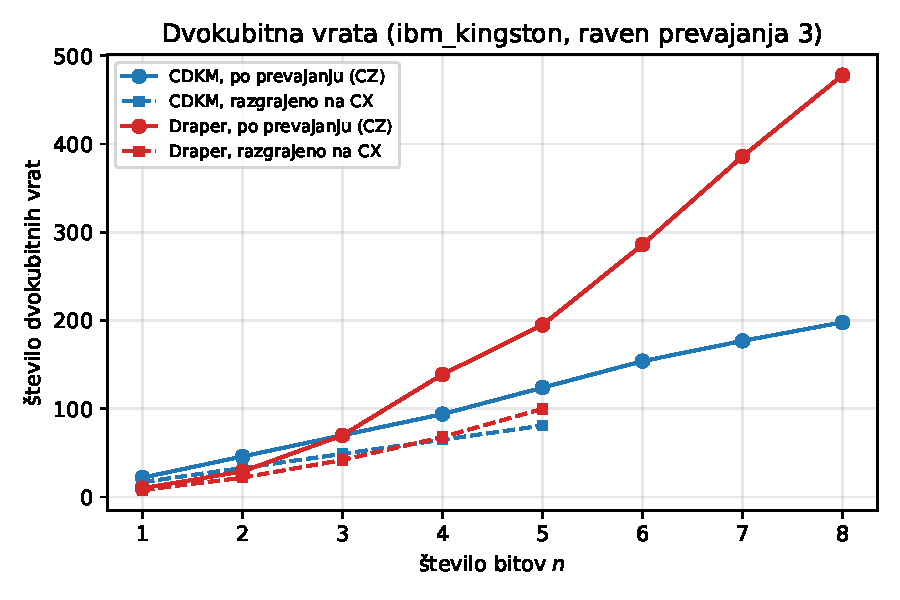
\includegraphics[width=\textwidth]{vrata}
\end{column}
\end{columns}
\end{frame}

% ---------------------------------------------------------------
\begin{frame}{Metoda}
\begin{itemize}
  \item Qiskit 2.6.2, Qiskit Aer 0.18.4, Qiskit Runtime (Sampler V2), Open Plan
  \item Pari vhodov: vsi pri $n \le 2$, 16 naključnih (fiksno seme) pri $n \ge 3$
  \item 1000 ponovitev na vezje
  \item Prevajanje: \texttt{optimization\_level=3}, \texttt{seed\_transpiler=2026}
  \item Idealni in šumni simulator (FakeTorino, FakeFez)
  \item Procesorja \textbf{ibm\_fez} ($n = 1$--$5$) in \textbf{ibm\_kingston} ($n = 1$--$8$), Heron r2
  \item Brez blaženja napak; dinamično razklapljanje (DD, XpXm) izklopljeno ali vklopljeno
  \item Oba seštevalnika v istem opravilu $\Rightarrow$ enaka kalibracija; 7 opravil
  \item Metrika: verjetnost pravilne vsote; napovedovalci: 2q vrata, ESP, globina, čas
\end{itemize}
\end{frame}

% ---------------------------------------------------------------
\begin{frame}{Simulator in procesor}
\begin{columns}[c]
\begin{column}{0.36\textwidth}
\begin{itemize}
  \item Idealni simulator: vedno pravilna vsota
  \item Šumni simulator: CDKM boljši od $n = 3$ ali $4$ naprej
  \item Procesor precej slabši: CDKM pri $n = 5$ \\ \slabo{27~\%} namesto 69~\%
\end{itemize}
\end{column}
\begin{column}{0.62\textwidth}
\centering
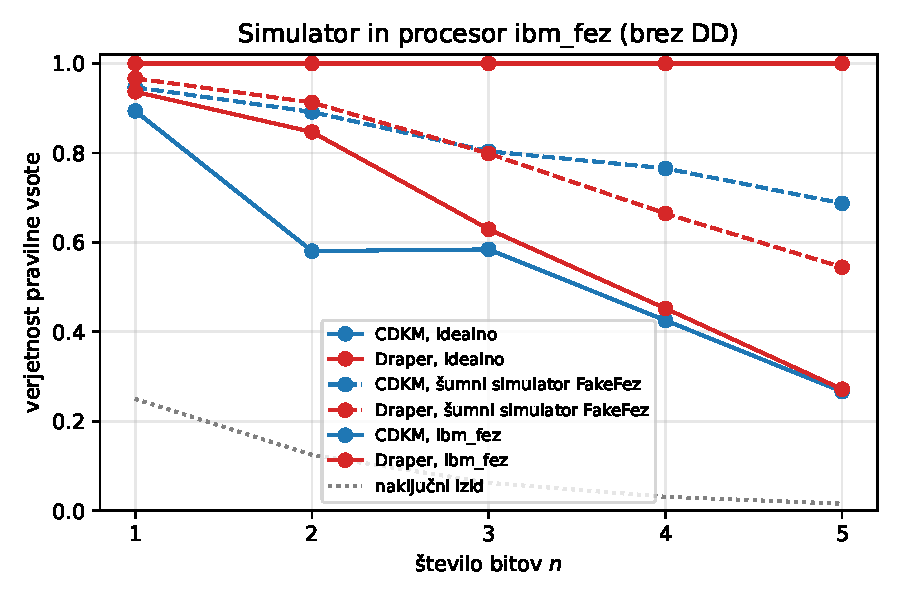
\includegraphics[width=\textwidth]{uspesnost_fez}
\end{column}
\end{columns}
\end{frame}

% ---------------------------------------------------------------
\begin{frame}{Vpliv dinamičnega razklapljanja}
\centering
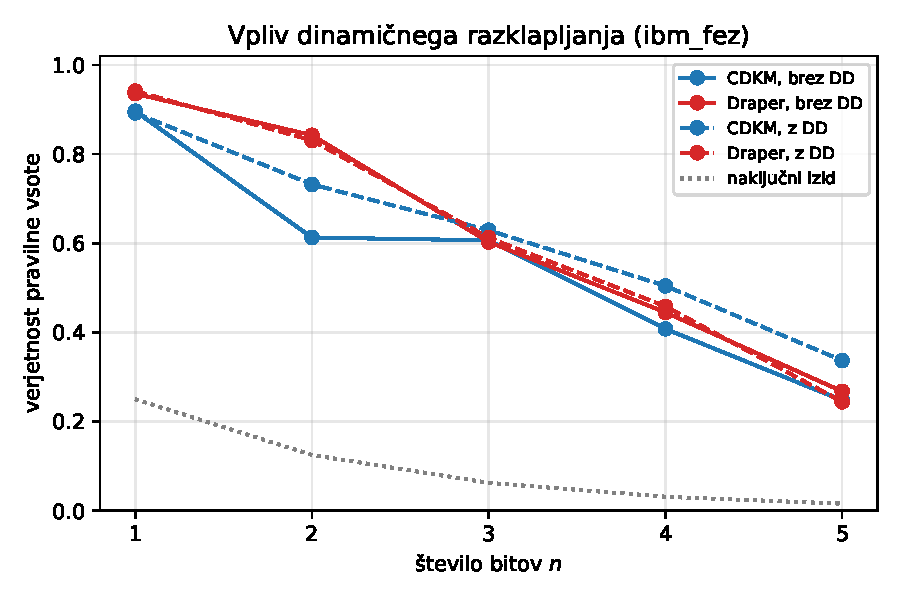
\includegraphics[width=0.49\textwidth]{dd_fez}\hfill
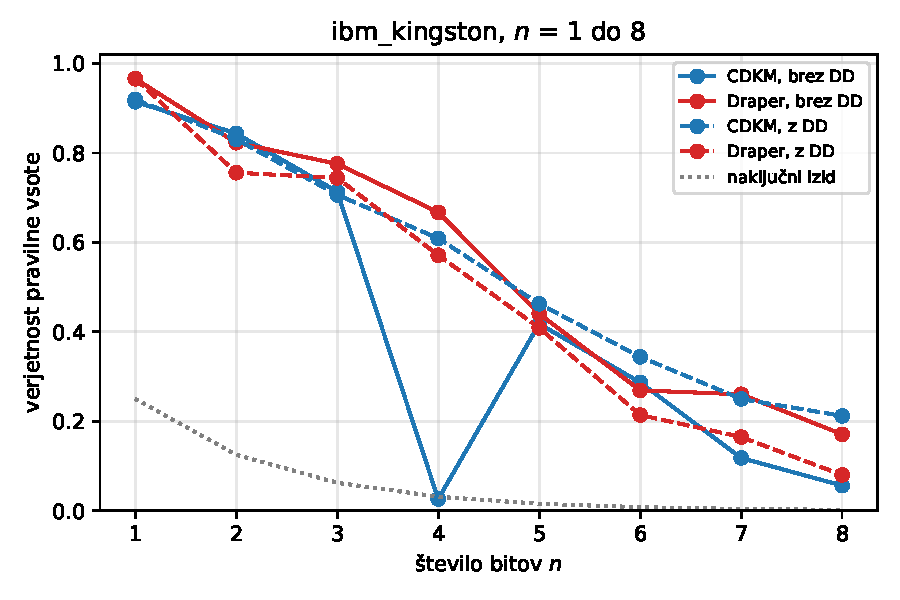
\includegraphics[width=0.49\textwidth]{kingston_n8}

\vspace{0.1cm}
{\small Polna črta: brez DD, črtkana: z DD.
Brez DD je Draper boljši ali enako dober pri večini $n$; z DD je CDKM boljši pri vseh $n \ge 4$.}
\end{frame}

% ---------------------------------------------------------------
\begin{frame}{Ali število vrat napove zmagovalca?}
Pri $n \ge 4$, kjer ima CDKM jasno manj vrat:
\vspace{0.3cm}
\begin{center}
\begin{tabular}{lcc}
\toprule
 & napoved velja & ibm\_kingston, $n = 8$ (CDKM / Draper) \\
\midrule
brez DD & \slabo{1 od 9} primerjav & 0,056 / 0,171 \\
z DD    & \dobro{7 od 7} primerjav & 0,212 / 0,080 \\
\bottomrule
\end{tabular}
\end{center}
\vspace{0.3cm}
\begin{itemize}
  \item DD izboljša CDKM pri večini $n$ (na ibm\_fez za največ 0,12), Draperju ne pomaga
  \item Hipoteze \alert{ne moreva potrditi}: velja le z DD
  \item Ne drži niti predpostavka: pri $n = 2$ ima CDKM več vrat, pri $n = 3$ enako
\end{itemize}
\end{frame}

% ---------------------------------------------------------------
\begin{frame}{Zakaj DD pomaga CDKM}
\small
\begin{itemize}
  \item Zaporedni prenos: kubiti dolgo čakajo ($n = 5$, ibm\_fez: mirovanje 83~$\mu$s proti 69~$\mu$s) $\Rightarrow$ dekoherenca in koherentne napake zaradi sklopitve ZZ
  \item ESP in število vrat tega ne zajameta, DD pa te napake zaduši
  \item Izmerjeno / ESP: brez DD CDKM 50--58~\%, Draper 71--73~\%; z DD oba 63--72~\% ($r = 0{,}94$--$0{,}97$)
\end{itemize}
\centering
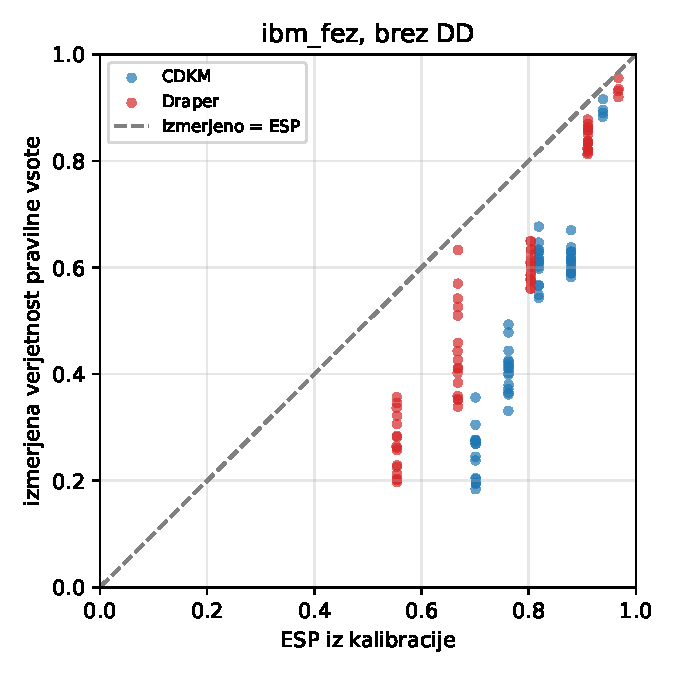
\includegraphics[height=0.43\textheight]{esp_brez_dd}\hspace{1cm}
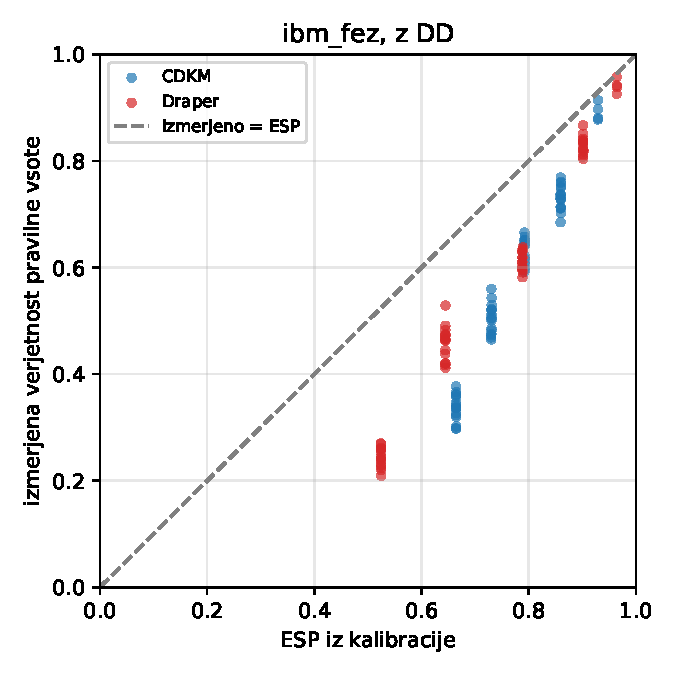
\includegraphics[height=0.43\textheight]{esp_dd}

\end{frame}

% ---------------------------------------------------------------
\begin{frame}{Kaj ni delovalo in omejitve}
\small
\begin{itemize}
  \item \textbf{Izstopajoč rezultat}: ibm\_kingston, CDKM, $n = 4$, brez DD: 2,6~\% (naključno 3,1~\%)
  \begin{itemize}
    \item napačen vedno isti bit $s_3$ (kubit 79), ESP napove 0,81
    \item z DD dve minuti pozneje na istih kubitih 0,61 $\Rightarrow$ verjetno koherentna napaka med mirovanjem
  \end{itemize}
  \item \textbf{Šumni simulator} ni napovedal izidov na procesorju (kolikor nama je znano, ne modelira presluha in napak med mirovanjem)
  \item \textbf{Metrika pred prevajanjem} je zavajala: ne zajame trokubitnih Toffolijevih vrat
  \item \textbf{Omejitve}: dva procesorja iste vrste, razlike med zagoni do 0,03, le 16 od $4^n$ parov vhodov
\end{itemize}
\end{frame}

% ---------------------------------------------------------------
\begin{frame}{Zaključek}
\begin{itemize}
  \item CDKM ima po prevajanju od $n = 4$ naprej manj dvokubitnih vrat (pri $n = 8$ 2,4-krat manj)
  \item Ta prednost se na procesorju pokaže \alert{le z dinamičnim razklapljanjem}
  \item Število dvokubitnih vrat je dober napovedovalec šele, ko so zadušene napake med mirovanjem
  \item Nadaljnje delo: ponovitve ob različnih urah, aproksimativna QFT, blaženje napak pri meritvah, seštevalnik z vnaprejšnjim izračunom prenosa
\end{itemize}
\end{frame}

% ---------------------------------------------------------------
\begin{frame}{Doprinosi avtorjev}
\begin{columns}[T]
\begin{column}{0.48\textwidth}
\textbf{Jurij Anžič}
\begin{itemize}
  \item seštevalnik CDKM in testi
  \item skupna koda: priprava vezij, prevajanje, metrike, simulatorji
  \item osnutek poročila
\end{itemize}
\end{column}
\begin{column}{0.48\textwidth}
\textbf{Janez Koprivec}
\begin{itemize}
  \item prijava teme, razvojno okolje
  \item Draperjev seštevalnik in testi
  \item zagon in poskusi na procesorjih IBM, analiza opravil
\end{itemize}
\end{column}
\end{columns}
\vspace{0.5cm}
\centering Oba: interpretacija rezultatov
\end{frame}

% ---------------------------------------------------------------
\begin{frame}[standout]
Hvala za pozornost!

\vspace{0.5cm}
\normalsize Vprašanja?
\end{frame}

\end{document}
